
关于C++内存管理的主题可以单独成书。关于STL分配器的问题,的论文很多。本章中,将重点讨论几个影响性能的问题。有些有简单的解决方案。其他的,我们将描述问题,并概述可能的解决方法。 

性能方面可能会遇到两种与内存相关的问题。第一个问题是使用太多内存:程序要么耗尽内存,要么没有满足内存使用要求。第二个问题发生在程序受到内存限制时,性能受到内存访问速度的限制。在这样的情况下,程序的运行时间与使用的多少内存直接相关,减少内存使用会使程序运行得更快。 

本节中介绍的示例适用于处理内存限制程序或频繁和/或大量分配内存的程序。我们从内存分配本身对性能的影响开始。

\subsubsubsection{9.4.1\hspace{0.2cm}不必要的内存分配}

与内存使用相关的性能问题之一是\textit{不必要的内存分配}。下面是一个常见的问题,用类似C++的伪代码来描述:

\begin{lstlisting}[style=styleCXX]
for ( … many iterations … ) {
	T* buffer = allocate(… size …);
	do_work(buffer); // Computations use memory
	deallocate(buffer);
}
\end{lstlisting}

良好的程序会使用RAII类来管理回收内存,但是为了清晰明了,希望使显式分配和回收。分配通常隐藏在管理自己内存的对象中,比如STL容器。这样会将大部分时间花在内存分配和回收函数(如\texttt{malloc()}和\texttt{free()})上。 

可以在基准测试中看到它对性能的影响:

\hspace*{\fill} \\ %插入空行
\noindent
\textbf{04\_buffer.C}
\begin{lstlisting}[style=styleCXX]
void BM_make_str_new(benchmark::State & state) {
	const size_t NMax = state.range(0);
	for (auto _: state) {
		const size_t N = (random_number() % NMax) + 1;
		char * buf = new char[N];
		memset(buf, 0xab, N);
		delete[] buf;
	}
	state.SetItemsProcessed(state.iterations());
}
\end{lstlisting}

这里是通过初始化一个字符串来表示的,\texttt{random\_number()}返回随机整数值(可能只是\texttt{rand()},但是若预先计算和存储随机数,以避免对随机数生成器进行基准测试,那么基准测试会更简洁)。可能还需要哄骗编译器不要优化掉结果,若\texttt{benchmark::DoNotOptimize()}不能满足要求,可能需要插入一个\texttt{print}语句,但条件永远不会发生(但编译器并不知道),比如\texttt{rand() < 0}。

从基准中得到的数据没什么意义,需要与其他东西进行比较才可以。我们的例子中,基线很容易确定,可以做相同的工作,但不进行分配。这可以通过将分配和回收移出循环来实现(已知最大内存大小):

\hspace*{\fill} \\ %插入空行
\noindent
\textbf{04\_buffer.C}
\begin{lstlisting}[style=styleCXX]
char * buf = new char[NMax];
for (auto _: state) {
	…}
delete[] buf;
\end{lstlisting}

基准测试中,观察到的性能差异在很大程度上取决于操作系统和系统库,但很可能会看到这样的情况(使用的是随机大小为1KB的字符串):

%\hspace*{\fill} \\ %插入空行
\begin{center}
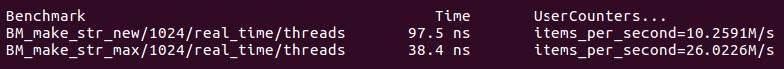
\includegraphics[width=0.9\textwidth]{content/3/chapter9/images/5.jpg}\\
图9.5 - 分配-回收模式对性能的影响
\end{center}

与内存分配模式复杂得多的大型程序相比,微基准测试中的内存分配通常更高效,因此频繁的分配和回收在实际中的影响可能更大。即使在我们的微基准测试中,每次分配内存的实现运行速度只有一次分配最大可能内存量的版本的40\%。 

如果在计算过程中所需要的最大内存是已知的,那么预先分配内存并从一个迭代到下一个迭代进行重用,就是一个简单的解决方案。这个解决方案也适用于许多容器,对于\texttt{vector}或\texttt{deque}容器来说,利用调整容器大小不会缩小其容量的事实,可以在迭代开始之前预留内存。

如果事先不知道最大内存大小,解决方案就会复杂一些。这种情况可以使用仅增长的缓冲区来处理。下面是一个简单的缓冲区,只能增长:

\hspace*{\fill} \\ %插入空行
\noindent
\textbf{04\_buffer.C}
\begin{lstlisting}[style=styleCXX]
class Buffer {
	size_t size_;
	  std::unique_ptr<char[]> buf_;
	public:
	explicit Buffer(size_t N) : size_(N), buf_(
	new char[N]) {}
	void resize(size_t N) { 
		if (N <= size_) return;
		char* new_buf = new char[N];
		memcpy(new_buf, get(), size_);
		buf_.reset(new_buf);
		size_ = N;
	}
	char* get() { return &buf_[0]; }
};
\end{lstlisting}

同样,这段代码对于演示和探索都非常有用。实际中,可能会使用STL容器或自己的库类,但它们都应该具有增加内存容量的能力。可以通过简单地修改基准测试,来比较这个只增长的缓冲区和固定大小的预分配缓冲区的性能:

\hspace*{\fill} \\ %插入空行
\noindent
\textbf{04\_buffer.C}
\begin{lstlisting}[style=styleCXX]
void BM_make_str_buf(benchmark::State& state) {
	const size_t NMax = state.range(0);
	Buffer buf(1);
	for (auto _ : state) {
		const size_t N = (random_number() % NMax) + 1;     
		buf.resize(N);
		memset(buf.get(), 0xab, N);
	}
	state.SetItemsProcessed(state.iterations());
}
\end{lstlisting}

现实中,使用更智能的内存增长策略可能会得到更好的结果(比请求的内存增长稍微多一些,所以不必经常增加内存——大多数STL容器都采用这种策略)。但在我们的演示中,想让事情尽可能的简单。在同一台机器上,基准测试的结果如下:

%\hspace*{\fill} \\ %插入空行
\begin{center}
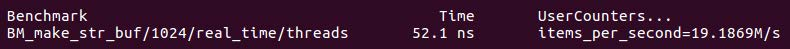
\includegraphics[width=0.9\textwidth]{content/3/chapter9/images/6.jpg}\\
图9.6 - 只增长缓冲区的性能(与图9.5相比)
\end{center}

只增长的缓冲区比固定大小的缓冲区慢,但比每次分配和回收内存都会快很多。同样,更好的增长政策将使这个缓冲更快,接近固定大小的速度。 

多线程程序中,良好的内存管理更为重要,因为对系统内存分配器的调用不能很好地扩展,并且可能涉及全局锁。同一台机器上使用8个线程运行基准测试会产生以下结果:

%\hspace*{\fill} \\ %插入空行
\begin{center}
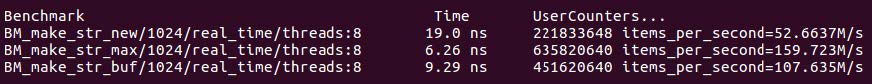
\includegraphics[width=0.9\textwidth]{content/3/chapter9/images/7.jpg}\\
图9.7 - 多线程程序中分配-回收模式对性能的影响
\end{center}

这里,频繁分配的代价更大(只增长缓冲区也展示了分配剩余内存的成本,从而从好的增长策略中受益)。 

尽可能少地与操作系统交互。如果有一个循环需要在每次迭代中分配和释放内存,那么在循环之前分配。如果分配的大小相同,或者预先知道最大分配大小,则预分配一个这个大小的内存,并保持它(当然,如果使用几个缓冲区或容器,不应该将它们硬塞到一个分配中,而是应该为每个区域进行预分配)。如果不知道最大内存大小,则使用可以增长的数据结构,但在工作完成之前不要缩减或释放内存。 

避免与操作系统交互的建议在多线程程序中尤为重要,现在我们将对并发程序中的内存使用做一些讨论。

\subsubsubsection{9.4.2\hspace{0.2cm}并发程序中的内存管理}

操作系统提供的内存分配器是一种平衡多种需求的解决方案。在给定的机器上,只有一个操作系统,但有许多不同的程序,它们有自己独特的需求和内存使用模式,开发人员非常努力地让它在合理的使用方式中不会失败。另一方面,它也很少是最佳解决方案。通常,这已经足够好了,特别是如果需要频繁的申请内存。

在并发程序中,内存分配变得更加低效。主要原因是,内存分配器都必须维护相当复杂的内部数据结构,以跟踪分配和释放内存。在高性能分配器中,内存会细分为多个方面,以便将类似大小的分配组合在一起。这就是以复杂性为代价,提高了性能。如果多个线程同时分配和释放内存,那么内部数据的管理必须由锁来保护。这是一个全局锁,用于整个程序,如果经常调用分配器,它会限制整个程序的扩展性。

这个问题最常见的解决方案是使用带有线程局部缓存的分配器,比如流行的\texttt{malloc()}替换库TCMalloc。这些分配器为每个线程预留了一定数量的内存,当一个线程需要分配内存时,首先从线程本地内存域中获取。这并不需要锁,因为只有一个线程与该域交互。只有当域为空时,分配器才必须从所有线程共享的内存中获取锁并进行分配。当一个线程释放内存时,释放的内存会添加到线程特定域中,同样不需要任何锁。

线程本地缓存也不是没有问题。

首先,它们倾向于使用更多的内存。如果线程释放了大量内存,而另一个线程分配了大量内存,那么最近释放的内存对另一个线程来说是不可用的(对于释放它的线程来说内存是本地的)。因此,当未使用的内存可供其他线程使用时,会分配更多的内存。为了限制这种内存浪费,分配器通常不允许每个线程的空间增长超过某个预定义的限制。达到限制时,线程本地内存将返回到所有线程共享的内存域中(这个操作需要一个锁)。

其次,如果每个分配都由一个线程拥有,这些分配器可以工作得很好,相同的线程可以在每个地址分配和释放内存。如果一个线程分配了一些内存,另一个线程必须释放,因为内存必须从一个线程的局部域,转移到另一个线程的局部域(或共享域),所以这种跨线程释放很困难。基准测试表明,使用标准分配器(如\texttt{malloc()}或TCMalloc)的跨线程回收的性能,至少比线程分别拥有本地内存的性能差一个数量级。对于使用线程本地缓存的分配器来说,这可能都是正确的,因此应该尽可能避免线程之间的内存交互。

现在,我们讨论的是将内存从一个线程传输到另一个线程,目的是回收内存。那么简单地使用由另一个线程分配的内存呢?这种内存访问的性能在很大程度上取决于硬件能力。对于CPU较少的简单系统,这可能不是问题。但是较大的系统有多个内存库,并且CPU和内存之间的连接是不对称的。每个内存库更接近一个CPU,这就是所谓的\textbf{非均匀内存访问(NUMA)}。NUMA对性能的影响差别很大,\textit{从无关紧要到快了一倍}。有一些方法可以优化NUMA内存系统的性能,并使程序内存管理对NUMA敏感。但请注意,您可能会针对特定的机器调优性能,但关于NUMA系统的一般性性能资料,可以几乎没有。

我们现在回到更有效地使用内存的问题,因为它对并发程序和串行程序的性能都有帮助。

\subsubsubsection{9.4.3\hspace{0.2cm}避免内存碎片}

困扰许多程序的问题是与内存分配系统的低效交互。假设程序需要分配1KB的内存。这个内存块是从一些更大的内存空间中取出来的,标记为由分配器使用,并将地址返回给调用者。接下来会分配更多的内存,所以1KB块之后的内存现在也使用了。然后程序返回第一个分配,并立即请求2KB的内存。这时有一个1KB的空闲块,但它不够大,不能满足新的请求。其他地方可能还有另一个1KB的块,但只要这两个块不是紧挨着的,则对于2KB的分配申请就没什么意义:

%\hspace*{\fill} \\ %插入空行
\begin{center}
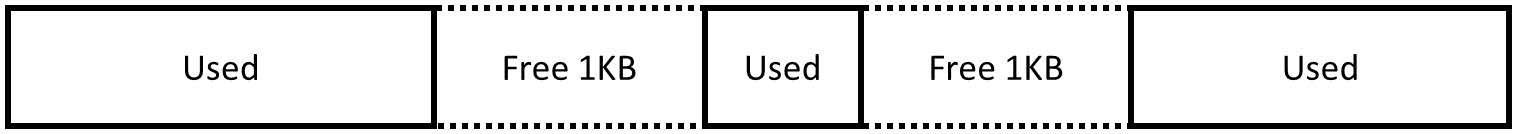
\includegraphics[width=0.9\textwidth]{content/3/chapter9/images/8.jpg}\\
图9.8 - 内存碎片:存在2KB的空闲内存,但对于单个2KB的分配并没啥用
\end{center}

这种情况称为\textbf{内存碎片}:系统有程序返回的空闲内存,但必须使用新的内存来服务于下一次分配,因为程序释放的内存分割成小块。在极端的情况下,这种碎片可能会导致程序在系统的总内存容量耗尽之前就“耗尽内存”(作者所见过的最糟糕的情况是,一个程序在只分配了总可用内存的1/6后就“耗尽”了内存)。有些内存分配器比标准的\texttt{malloc()}更能抗碎片,但是对于快速移动内存的程序,可能需要更极端的措施。

一种解决方式为块分配器,所有内存都以固定大小的块(比如64KB)分配。不能从操作系统一次分配一个这样大小的块,而是分配较大的内存块(例如,8MB),并将它们细分为较小的块(在我们的示例中为64KB)。处理这些请求的内存分配器是程序中的主分配器,直接与\texttt{malloc()}交互。因为只分配一个大小的块,所以非常简单,这样我们就可以专注于最有效的实现(并发程序的线程本地缓存,实时系统的低延迟等)。当然,谁都不想在代码中处理这些64KB的块(其实这是二级分配器的工作),如图9.9所示:

%\hspace*{\fill} \\ %插入空行
\begin{center}
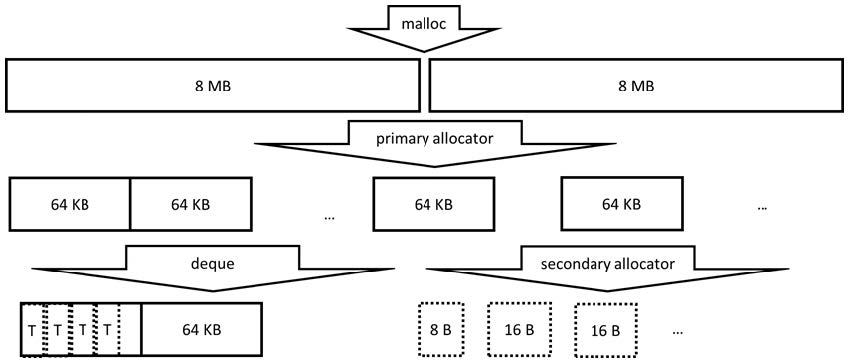
\includegraphics[width=0.9\textwidth]{content/3/chapter9/images/9.jpg}\\
图9.9 - 固定大小的块分配
\end{center}

可以使用分配器将64KB的块进一步细分为更小的块。统一分配器(只分配一个大小的分配器)非常高效,为单个64位整数分配内存,就可以这样做,而不需要任何内存开销(相比之下,\texttt{malloc()}每次分配通常需要至少16个字节的开销)。还可以使用容器以64KB块分配内存,并使用它来存储元素。这里不会使用\texttt{vector},因为它需要一个大型的、连续的分配。这里需要的容器是\texttt{deque},它在固定大小的块中分配内存。当然,也可以使用节点容器。如果STL分配器接口足以满足需求,可以使用STL容器,要不就需要编写自己的容器库了。

固定大小的块分配的优点是不会受到碎片化的影响,\texttt{malloc()}的所有分配都是相同的大小,主分配程序的所有分配也是一样的。一个内存块返回给分配器时,都可以重用以满足下一个内存请求。参考下图:

%\hspace*{\fill} \\ %插入空行
\begin{center}
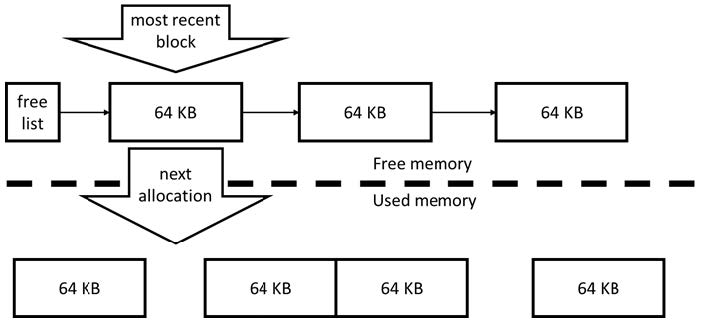
\includegraphics[width=0.9\textwidth]{content/3/chapter9/images/10.jpg}\\
图9.10 - 固定大小分配器中的内存重用
\end{center}

这种先进先出的属性也是一个优势。最后的64KB内存块很可能来自最近使用的内存,并且在缓存中仍然是\textit{热的}。重用这个块可以立即改善内存引用的局部性,因此可以更有效地使用缓存。分配调度器会返回块作为一个简单的空闲链表(图9.10)。可以为每个线程维护这些空闲链表,以避免锁的使用,可能需要定期重新平衡,以避免线程积累了过多的空闲块,而另一个线程正在分配新内存的情况。

当然,将64KB块细分成更小大小的分配器时,仍然容易受到碎片的影响,除非也是统一(固定大小)的分配器。然而,如果必须处理较小的内存(一个块)和少量不同大小的内存,那么编写一个可以自动进行碎片整理分配器会更容易。 

使用块内存分配的决定很可能会影响整个程序,例如:分配大量的小数据结构,使每个数据结构使用64KB块的一小部分,这将降低内存的性价比。另一方面,如果数据结构本身是一组较小的数据结构(容器)的集合,可以将许多较小对象打包到一个块中,那么这种数据结构就更容易处理。甚至可以编写压缩容器来压缩每个块,以便长期保存数据,然后进行解压缩以便访问。 

区块大小本身也不是一成不变的。一些应用程序使用更小的块会更有效率,如果块部分未使用,内存浪费更少。其他线程可以减少大内存块分配的次数,从而在性能上获益。

关于特定于应用程序的分配器的文献非常丰富,例如:slab分配器是刚才看到的块分配器的泛化版本,可以有效地管理多个内存分配。还有许多其他自定义的内存分配器,其中大多数都可以在C++中使用。特定应用程序的分配器通常会带来显著的性能改进,但代价通常是严重限制了开发者实现数据结构的自由。

下一个导致效率低下的常见原因更为微妙,也更难处理。





















